
\section{Underlying concepts and theoretical formulation}
\secL{statement_of_the_problem}

In this section we provide the concepts and the formal
definitions that we will use later to express PS, the algorithm we
propose.  First, we give the definitions of Pareto set and Pareto
front that lie on the basis of Design Space Exploration.
Then, we sketch the fundamental idea behind our algorithm. Finally, we
provide a formal definition of the regions, of their properties and of
the operations that will be performed on them by the algorithm.

In this section and the following one, we will deliberately keep our formulation as general as possible, even if the focus of this paper is the embedded system design space exploration. The goal is to make the generality of PS emerge. We argue that it is a strong point for PS, as for genetic algorithms, since (i) it permits to apply it to a wide range of different problems and (ii) it can be effectually used when the embedded system design is particularly challenging and no much a-priori knowledge is available to the designer. As already pointed in \secL{related_work}, the generality of genetic algorithms has made them widely deployed with respect to the other approaches.
Thanks to the generality of PS, we will not need to modify or adapt it in order to apply it to the case of embedded system design, as we will show in \secL{ee}. On the one hand, this legitimate our choice of keeping formulation general. On the other hand, more importantly, this confirms the capability of PS to automatically adapt to the problem under investigation, without any explicit intervention or knowledge of the designer, required, on the contrary, by~\cite{givargis_tvlsi02,santosh_hptr00,dellnitz2005covering} .

\subsection{Pareto set and Pareto front}
\secL{pareto}

Let $S$ be a parameterized system with $n$ parameters. The generic
parameter $p_i, \ i \in \{1,2,\ldots,n\}$ can take any value in
the set $V_i$. A {\em configuration} $\mathbf{c}$ of the system
$S$ is a $n$-tuple $\langle v_1,v_2,\ldots,v_n \rangle$ in which
$v_i \in V_i$ is the value fixed for the parameter $p_i$. The {\em
configuration space} (or {\em design space}) of $S$ [which we will
indicate as $\mathcal{C}(S)$] is the complete range of possible
configurations [$\mathcal{C}(S) = V_1 \times V_2 \times \ldots
\times V_n$]. Naturally, not all the configurations of
$\mathcal{C}(S)$ can really be mapped on $S$, but only a subset 
is feasible. We call this subset {\em
feasible configuration space} of $S$ and indicate it as
$\mathcal{C}^*(S)$].

Let $m$ be the number of objectives to be optimized (e.g. power,
cost, performance, etc.). An {\em evaluation function}
$E:\mathcal{C}^*(S)\times \mathcal{B} \longrightarrow \Re^m$ associates each feasible configuration of $S$ to
an $m$-tuple of values corresponding to the objectives when any application belonging to the set of benchmarks
$\mathcal{B}$ is executed.

Given a system $S$, an application $b \in \mathcal{B}$ and two
configurations $\mathbf{c}', \mathbf{c}'' \in \mathcal{C}^*(S)$,
$\mathbf{c}'$ is said to {\em dominate} (or {\em eclipse})
$\mathbf{c}''$, if, given $\mathbf{o}'=E(\mathbf{c}', b)$ and
$\mathbf{o}''=E(\mathbf{c}'', b)$, it results that $\mathbf{o}'
\leq \mathbf{o}''$ and $\mathbf{o}' \neq \mathbf{o}''$, where
vector comparisons are interpreted component-wise and are true
only if all of the individual comparisons are true ($o'_i \leq
o''_i \ \forall \ i = 1,2,\ldots,m$). To indicate that 
$\mathbf{c}'$ dominates $\mathbf{c}''$, we use the notation
$\mathbf{c}' \succ \mathbf{c}''$.

\begin{definition}[Pareto set and Pareto front]
\defL{pareto-set}
The {\em Pareto-optimal set} of $S$ (or, shortly, Pareto-set) for the application $b$ is the
set:
\[ \mathcal{P}(S,b) = \left\{ \mathbf{c} \in \mathcal{C}^*(S) \ | \nexists \ \mathbf{c}' \in \mathcal{C}^*(S), \mathbf{c}' \succ \mathbf{c} \right\} \]
\end{definition}
that is, the set of configurations $\mathbf{c} \in
\mathcal{C}^*(S)$ not dominated by any other configuration.
The configurations belonging to the Pareto-optimal set are called \emph{Pareto-optimal configurations}, while the {\em Pareto-optimal front} (or, shortly, Pareto-front) is their image, i.e. the set:
\[ \mathcal{P}_{F}(S,b) = \{ \mathbf{o} | \mathbf{o} = E(\mathbf{c},b), \mathbf{c} \in \mathcal{P}(S,b) \} \]

Another fundamental concept, which adds further complexity to the
problem of multiobjective design space exploration, is the following

\begin{definition}[Parameter dependencies]
\defL{dependency}
Given a system $S$, application $b \in \mathcal{B}$ and two parameters
$p_x$ and $p_y$, $p_x$ is said to
be dependent on another parameter $p_y$ if the optimal value of $p_x$,
that is the $v_{x} \in V_x$ which optimizes the objectives of the
evaluation function $E$, is dependent upon the current value of $p_y$. 
\end{definition}

When a dependency is present any safe assumption about the ``meaning'' of
$p_x$ in order to intuitively choose an appropriate value that
optimizes objective could be misleading.  It should be also pointed
out that it's often very difficult to identify dependencies using
analytical techniques and often designers have to use different
strategies to deal with such complexity, as seen
in~\secR{Related-work}.

The aim of a Design Space Exploration (DSE) strategy is to give a
good approximation of the Pareto-optimal set for a system $S$ and an
application $b$, simulating as few configurations as possible.
As we will show later, at each iteration, PS calculates an approximation $\mathscr{P}_i$ of the Pareto-set that approaches it as iterations go on. The image of $\mathscr{P}_i$ is an approximation of the Pareto-front.
The simulation effort is distributed more on the regions that provide configurations in $\mathscr{P}_i$ which introduce more \emph{innovation}, i.e. whose image in the objective space is more distant, thus ``more different'', from the previous Pareto-front approximation point.




% A PROPOSITO DI QUESTO DUBBIO:
%\comment{AA: Mi sembra solo un cambio di notazione. DP: c'era un On the contrary troppo aggressivio, ho cercato di alleggerire la cosa, ma dai un'occhiata }
% HO CANCELLATO TUTTA QUESTA PARTE.
% For each point of the Pareto front we can imagine the corresponding configuration as a point of $P_{1}\times\dots\times P_{n}$ space. We will also refer to these points as ``parameter space representation'' of the Pareto front. \figR{psos} shows the relation between the objective space (containing the Pareto front) and its parameter space representation. In particular in this work we are interested in the relation between the evolution of the points in the two spaces, e.g. how some properties of the Pareto front points can reflect some features of the corresponding points in the parameter space.

\begin{figure}[t]
\figLC{psos}{Relation between Pareto-set and Pareto front.}
\center
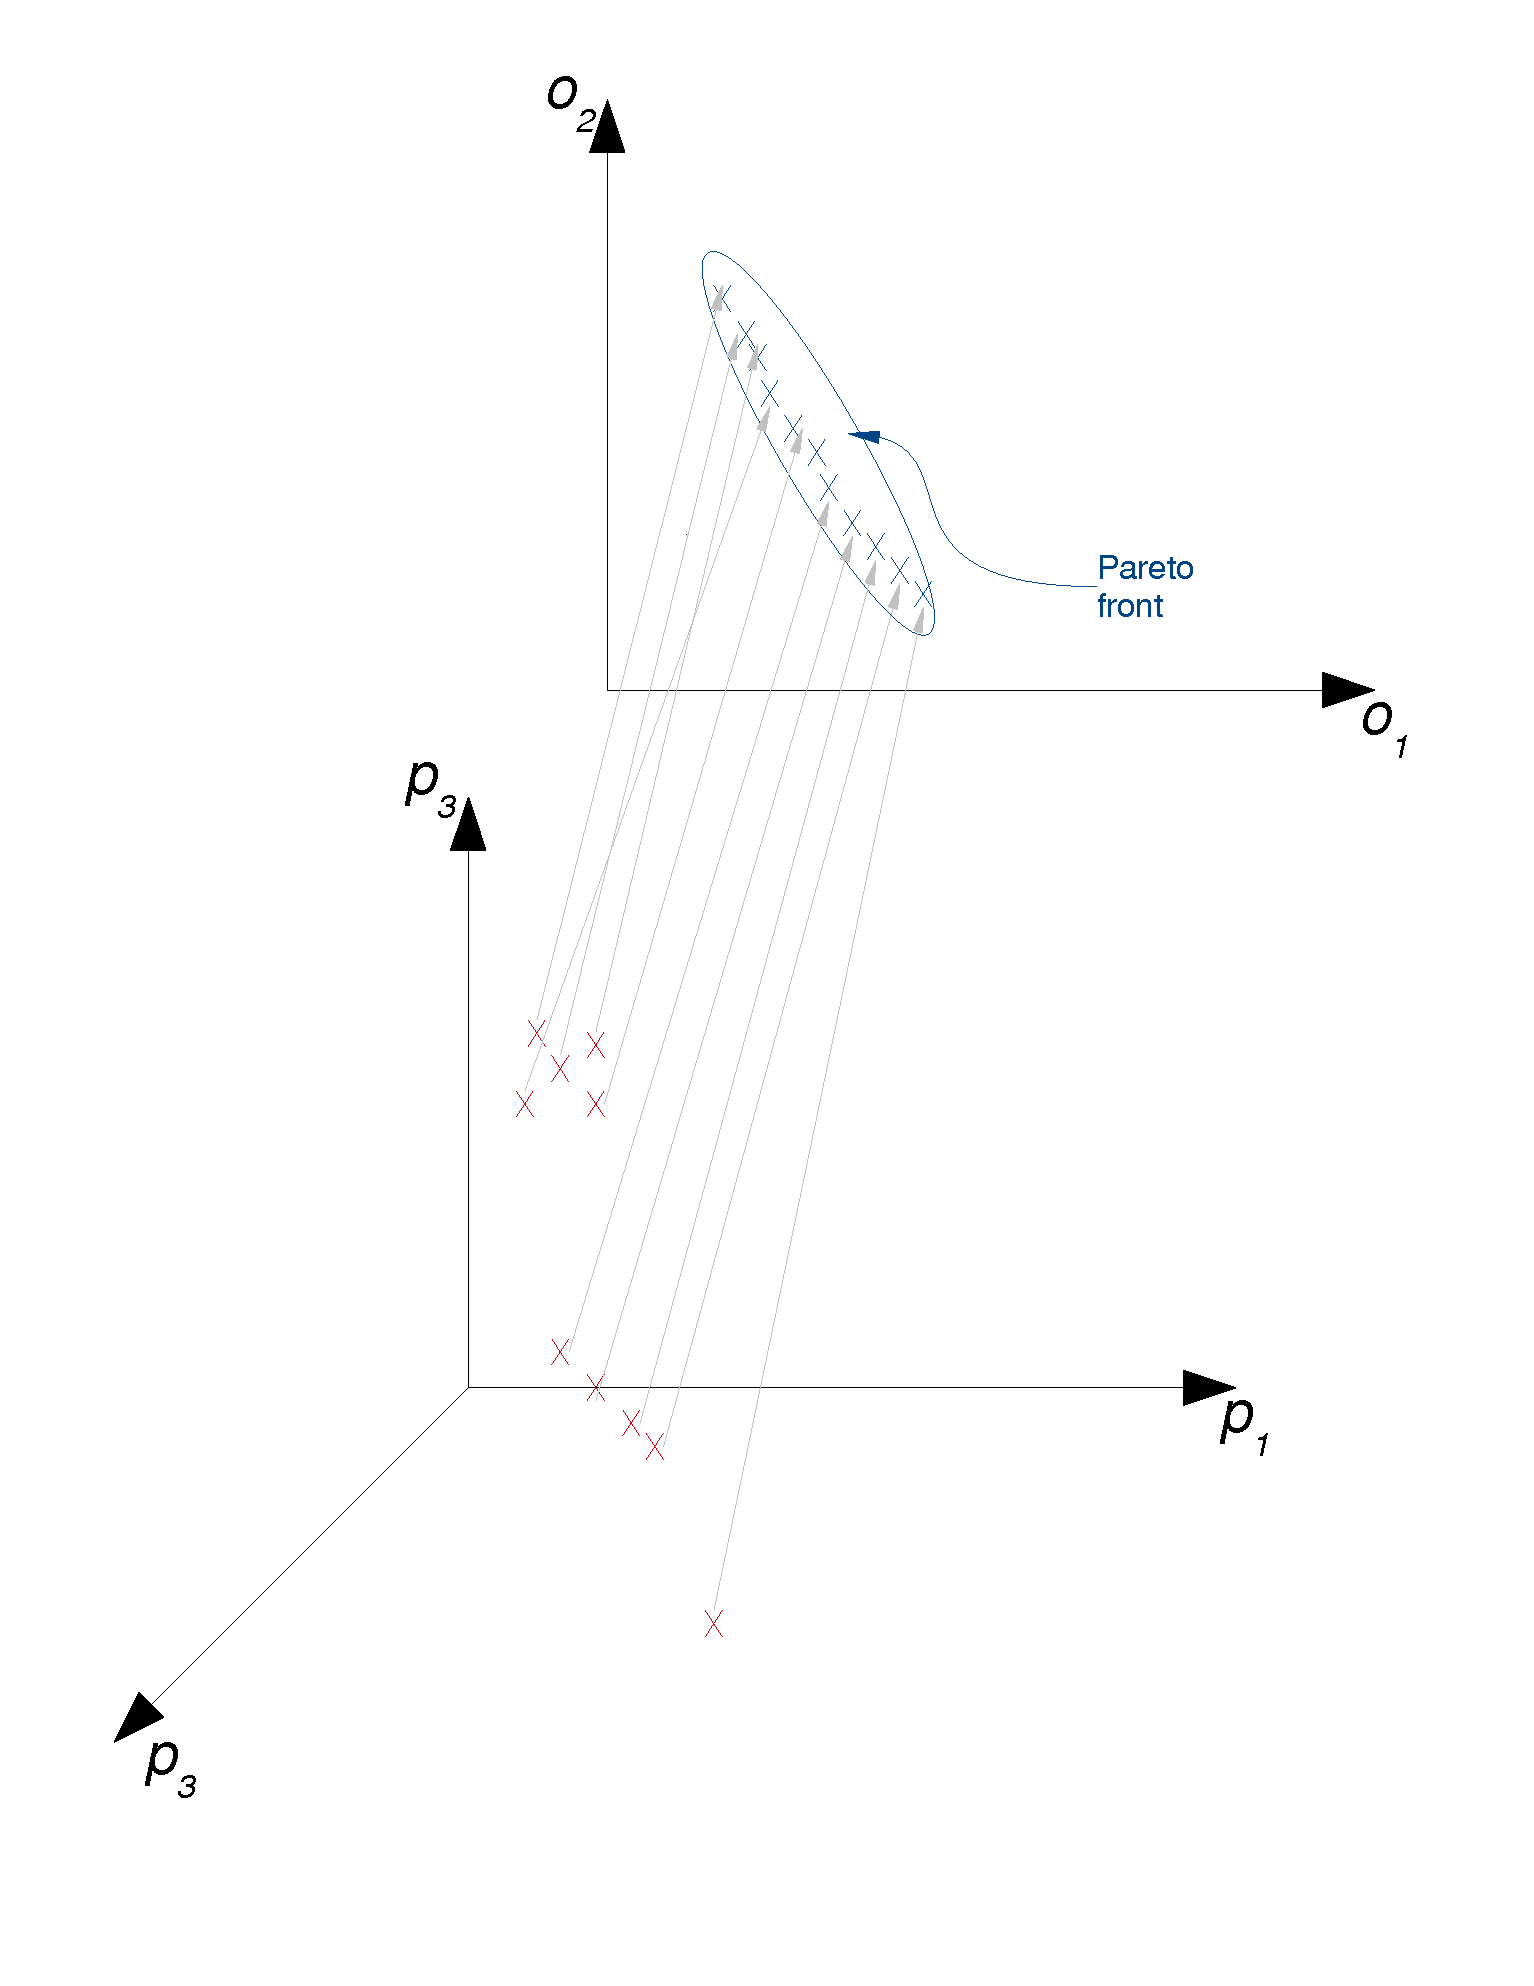
\includegraphics[width=0.5\columnwidth]{img/Pareto_set_and_front}
\end{figure}

\subsection{Sketch of the Idea}
\secL{sketch}

In the design process, there are often a lot of ``local decisions'' in
which the designer can take advantage of well-known results or
heuristics. For example, if we consider a highly parallel
computer architecture in a configuration with very few registers, it is
well-known that increasing the number of ALUs does not bring tangible
better performances but only cause an increase in area occupation. An
intelligent exploration algorithm would not waste time evaluating
configurations with many ALUs and few registers. If $p_{1}$ is the
parameter ``number of registers'' and $p_{2}$ is the parameter
``number of ALUs'', we can say that the region:
\[
R=\left\{ \left.\left(v_{1},v_{2}\right)\in P_{1}\times P_{2}\right|v_{1}<s_{1},v_{2}>s_{2}\right\} 
\]
 (where $s_{1}$ and $s_{2}$ are some threshold values) is \emph{uninteresting}. This clearly shows that there are cases when, if a parameter lies in
a certain range, there are ranges of the other one that are not worth being explored. Intuitively, the cartesian product of these ranges is an \emph{uninteresting region}.

The problem is that, in complex scenarios, not all the relations of this
kind are known in advance. Some dependency may be hidden
to the designer.
Therefore, as stated in \secR{Related-work},
setting up an exploration trying to take into account as much dependencies
as possible is a hard task that is destined to be incompletely
accomplished. We need a methodology to ``automatically'' recognize
interesting or uninteresting regions without requiring a priori knowledge
to the designer, that is what our algorithm does.

We also consider, in measuring how much interesting a region is, the
\emph{innovation} that it adds. If, during a design space exploration,
a Pareto front approximation is temporarily calculated, adding a new Pareto front
point near to the previous ones is not a considerable innovation,
because the way it fulfills the objectives is similar to the other
already evaluated configurations. On the contrary, adding a new Pareto
front point that is distant from previous ones is remarkable,
since it let the experimenter discover potential performance that have not yet considered before.
At each iteration, PS ``zooms in'' the most interesting regions while ``zooming out'' from the rest of configuration space. In order to implement this behavior algorithmically, at each iteration PS assigns the same number $N$ of simulations to each region. If a region $R$ is interesting, it is split in $k$ sub-regions before the next iteration starts. Therefore, in the next iteration, $N$ simulations are assigned to each sub-region. As a result, we are populating the original region $R$ with $k\cdot N$ simulations. On the contrary, uninteresting regions are merged, so that each one will receive less effort in the next iteration. In other words, ares of the configuration space that are more promising are split in small sub-regions, while the other ones are blended in big regions. As illustrated in \figR{small_and_big}, assigning $N$ simulations to each region makes small ones well populated while bigger ones sparsely explored.


	\begin{figure}[t]
	\center
	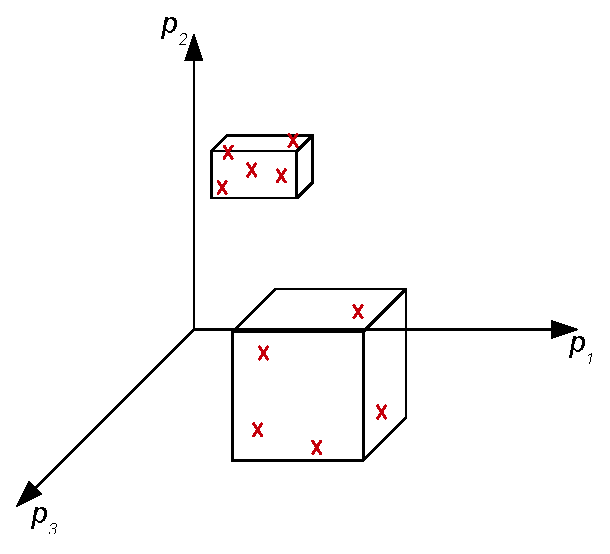
\includegraphics[width=0.5\columnwidth]{img/small_and_big}
	\figLC{small_and_big}{In this example 5 configurations
	are evaluated in a small region and in a bigger region. In can be
	seen that smaller region is more crowded.}
	\end{figure}


\subsection{Formal definitions}
We start by defining the parameter interval and the concept of interval contiguity. Using these definition we construct the region and define the region contiguity. Then we define the operations of splitting and merging regions. Finally, we provide the definition of separation.

Since regions will be defined as cartesian products of parameter intervals, we need the following definition.
\begin{definition}[Parameter interval] Let $p_{i}$ be a parameter and $a_{i},b_{i}\in V_{i},a_{i}<b_{i}$.
A $p_{i}$- interval is
	\[
	\left[a_{i}..b_{i}\right]=\left[a_{i},b_{i}\right]\cap P_{i}
	\]
i.e. taking the interval $\left[a_{i}..b_{i}\right]$
is the set of values of $V_{i}$ lying in $\left[a_{i},b_{i}\right]$)
\end{definition}


	\begin{figure}[t]
		\begin{center}
			\subfigure[Examples of contiguous and non contiguous intervals.]{
				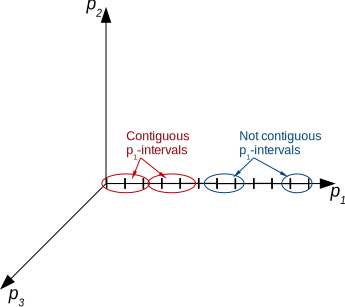
\includegraphics[width=0.45\textwidth]{img/contiguous_intervals_or_not} }
			\subfigure[Examples of regions.]{
				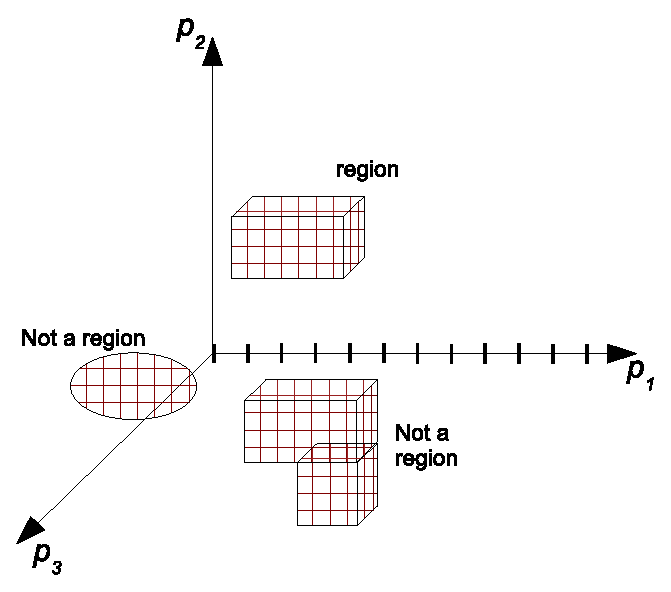
\includegraphics[width=0.45\textwidth]{img/regions} }
		    \figLC{interval_and_region}{Intervals and regions.}
		\end{center}
	\end{figure}



We consider only parameters $p_{i}$ with ordering, i.e. such
that $\forall a,b\in V_{i}$ it is possible
to say $a<b$ or $a=b$ or $a>b$. 
The following definition of interval contiguity will be the base of the concept of region contiguity, used to define merging and splitting operations.
\begin{definition}[Contiguous intervals]
\label{pers02.def:Contiguous-intervals}
Two intervals are contiguous iff they do not overlap and merging them results in a new interval. More formally, let $\left[a_{i}..b_{i}\right]$ and $\left[x_{i}..y_{i}\right]$
be two $p_{i}$-intervals. They are said to be contiguous (see \figR{interval_and_region}(a) ) iff
\begin{align}\begin{array}{l}
	\left[a_{i}..b_{i}\right]\cap\left[x_{i}..y_{i}\right]=\emptyset \mbox{      and} \\
	\left[a_{i}..b_{i}\right]\cup\left[x_{i}..y_{i}\right]$ is a $p_{i}$-
interval or $\left[x_{i}..y_{i}\right]\cup\left[a_{i}..b_{i}\right]
\end{array}\end{align}
\end{definition}

\begin{definition}[Region] 
A region is a cartesian product of parameter intervals, as illustrated in \figR{interval_and_region} (b). More formally, if $p_1,\dots,p_n$ are the parameters of the system, and $\left[ a_{i}..b_{i} \right]$ is a $p_i$-interval, a region is a set of the following form:
\[
R=\left[a_{1}..b_{1}\right]\times\dots\times\left[a_{n}..b_{n}\right]=\prod\left[a_{i}..b_{i}\right]
\]
\end{definition}

We will refer later to ``big'' and ``small'' regions. The sense
of these terms is related to the cardinality of regions.
\begin{definition}[Interval and region comparison]
A $p_{i}$-interval $\left[a_{i}..b_{i}\right]$
is said to be bigger then another $p_{i}$-interval $\left[c_{i}..d_{i}\right]$
iff 
$\left|\left[a_{i}..b_{i}\right]\right|>\left|\left[c_{i}..d_{i}\right]\right|$.
Similarly, a region $R_{1}$ is said to be \emph{bigger }then $R_{2}$, if
$\left|R_{1}\right|>\left|R_{2}\right|$
\end{definition}
Note that with $|\cdot|$ we indicate the cardinality of a set. Therefore, $\left|\left[a_{i}..b_{i}\right]\right|$ is the number of values of $V_i$ lying between $a_{i}$ and $b_{i}$ and has not to be confused with $b_i - a_i$.
Similarly $\left|R_{i}\right|$ is the number of configurations inside the region $R_i$.

As already explained, we will split interesting regions and merge uninteresting ones. The region splitting and merging operations are defined starting from the corresponding operations defined on intervals.
\begin{definition}[Splitting an interval]
\defL{splitting-a-region}
Given a $p_i$ interval $\left[a_{i}..b_{i}\right]$ with more than one element, i.e. $\left|\left[a_{i}..b_{i}\right]\right|>1$, the splitting operation produces as result two contiguous intervals $\left[a_{i}..c_{i}\right],\left[d_{i}..b_{i}\right]$
 such that
	\begin{align}
		\begin{cases}
		\left[a_{i}..c_{i}\right]\cap\left[d_{i}..b_{i}\right] & =\emptyset\\
		\left[a_{i}..c_{i}\right]\cup\left[d_{i}..b_{i}\right] & =\left[a_{i}..b_{i}\right]\\
		\left|\left[a_{i}..c_{i}\right]\right| & =\left\lceil \frac{\left|\left[a_{i}..b_{i}\right]\right|}{2}\right\rceil 
		\end{cases}
	\end{align}

We define the split operator $\psi$ as the one that, when applied to the intervals, gives the result of the split operation, i.e., in the case above, $\psi \left[a_{i}..b_{i}\right]=\lbrace \left[a_{i}..c_{i}\right],\left[d_{i}..b_{i}\right] \rbrace$.
If $\left|\left[a_{i}..b_{i}\right]\right|=1$, the interval
cannot be split and $\psi \left[a_{i}..b_{i}\right]=\left[a_{i}..b_{i}\right]$.
\end{definition}

The interval split is illustrated in \figR{split}~(a). Note that, when splitting an interval, the resulting intervals must satisfy two conditions: (i) they must be contiguous and, merging them, the initial interval must be obtained; (ii) the point in which we cut the interval is not arbitrary, but it is close to the middle.

\begin{definition}[Splitting a region]
\label{pers02.def:Splitting-a-region}
Consider a region $R=\prod\left[a_{i}..b_{i}\right]$.The split operator $\psi$ divides it into a set of sub-regions obtained splitting each $p_i$-interval and combining the resulting sub-intervals with the cartesian product, as shown in \figR{split}~(b). Formally:
	\begin{align}
		\psi(R) = \left\{ \left.\prod\left[x_{i}..y_{i}\right]\right|\left[x_{i}..y_{i}\right]\in \psi\left[a_{i}..b_{i}\right]  \right\} 
	\end{align}

\end{definition}


	\begin{figure}[t]
	    \figLC{split}{Split operations.}
		\begin{center}
			\subfigure[Splitting an interval.]{
				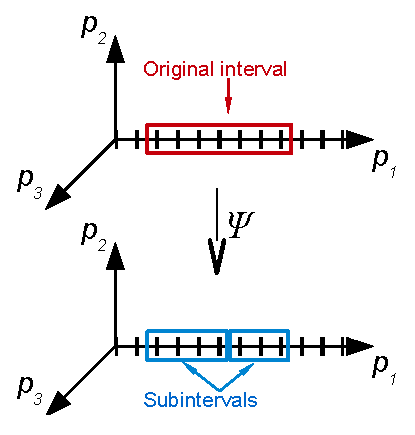
\includegraphics[width=0.30\textwidth]{img/splitting_intervals} }
			\subfigure[Splitting a region.]{
				\includegraphics[width=0.60\textwidth]{img/splitting_regions} }
		\end{center}
	\end{figure}


The merging operation will be defined only on region pairs that satisfy the conditions provided in the following definition.
\begin{definition}[Contiguous regions]Let $R_{1}=\prod\left[a_{i}\dots b_{i}\right]$ and $R_{2}=\prod\left[x_{i}..y_{i}\right]$
be two regions. They are said to be contiguous iff they do not overlap and, merging them, a new region can be obtained. Formally, $R_1$ and $R_2$ are contiguous iff there exists a $j$ such that:
	\begin{align}\begin{array}{l}
		\left[a_{i}..b_{i}\right]=\left[x_{i}..y_{i}\right]$
	\mbox{ for } $i\neq j \mbox{      and} \\
		\left[a_{j}..b_{j}\right]$ and $\left[x_{j}..y_{j}\right] \mbox{ are contiguous intervals}
	\end{array}\end{align}
\noindent We call $p_j$ the \emph{contiguity parameter} for the two regions.
\end{definition}

Examples of contiguous and non contiguous regions are given in \figR{contiguous_regions}. The two regions at the top are contiguous because their union can be expressed as the cartesian product of parameter intervals, thus they can be merged to obtain a new bigger region. The same also applies to the regions on the right. On the contrary, the two regions on the left (or of the two regions at the bottom) cannot be merged. 

	\begin{figure}[t]
		\center
		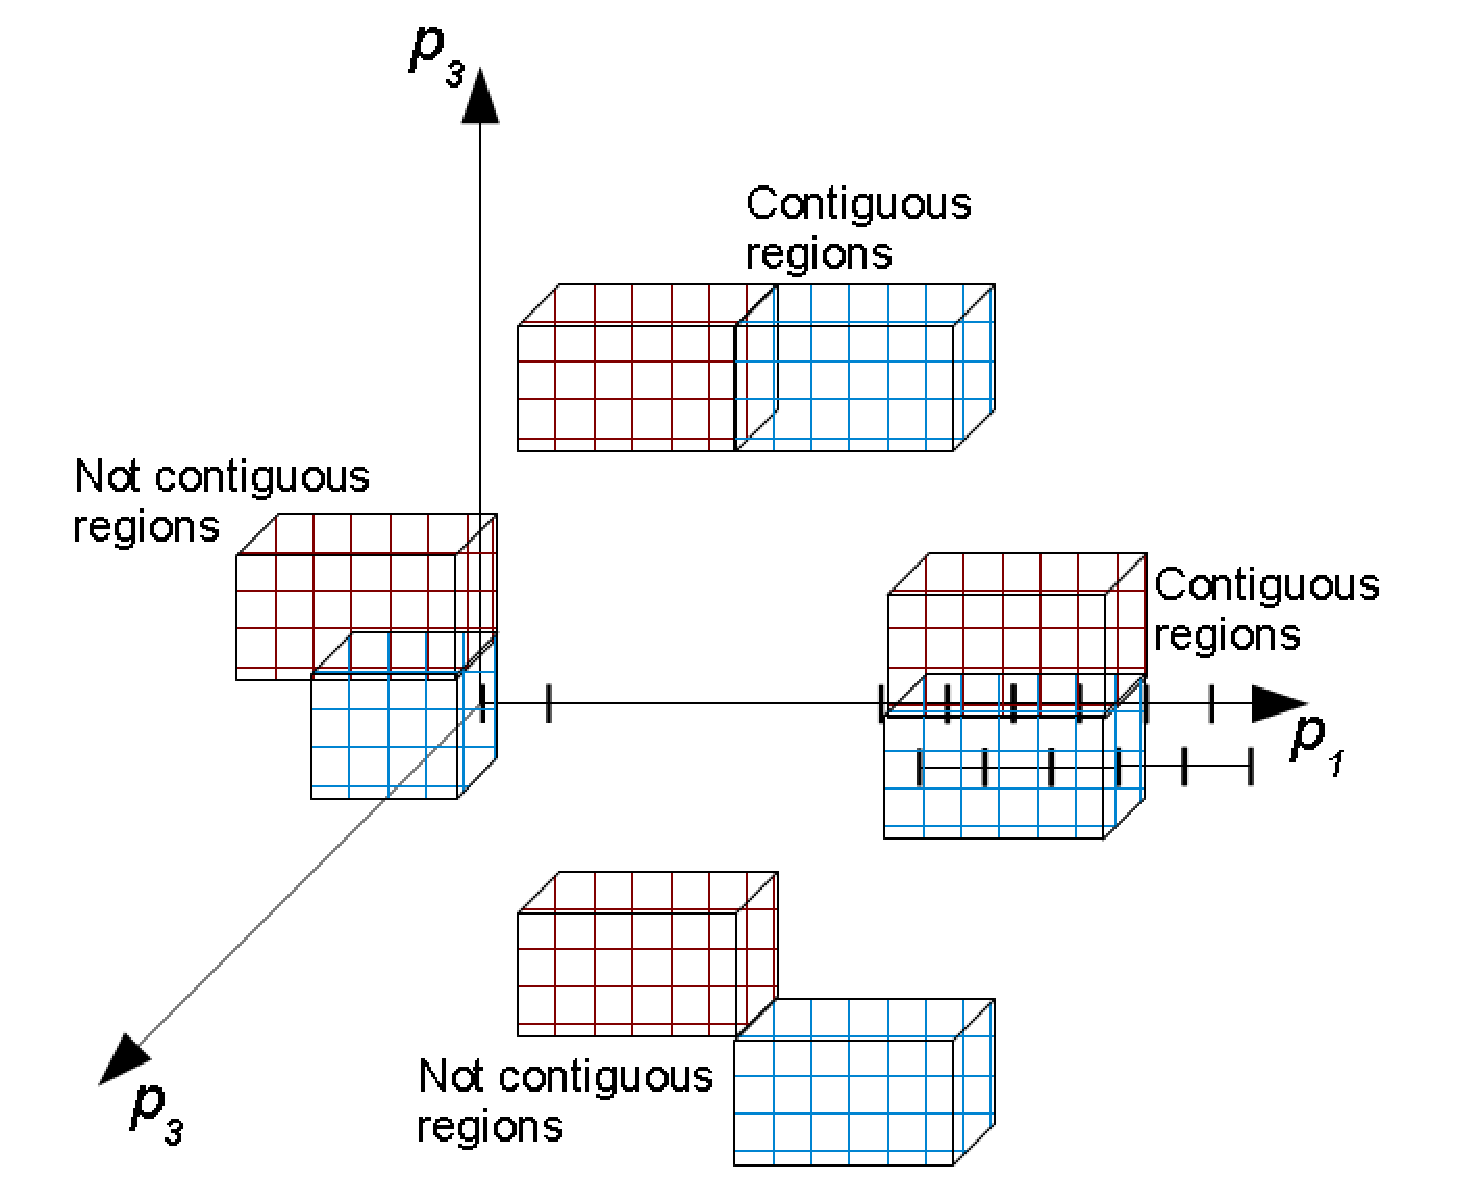
\includegraphics[width=0.8\columnwidth]{img/contiguous_regions}
		\figLC{contiguous_regions}{Contiguous and non contiguous regions.}
	\end{figure}

We now formally describe the merging operations.
\begin{definition}[Merging intervals]
Let $\left[a_{i}\dots b_{i}\right]$ and $\left[x_{i}..y_{i}\right]$ be two contiguous $p_i$-intervals. The merge operation applied to them produces a new $p_i$-interval of the following form:
	\begin{align}
		\mu	 \left( \begin{array}{l}
				\left[a_{j}..y_{j}\right] \\
				\left[x_{j}..b_{j}\right]
		     \end{array} \right)
		=\begin{cases}
			\left[a_{j}..y_{j}\right] & \mbox{ if }b_{j}<x_{j}\\
			\left[x_{j}..b_{j}\right] & \mbox{ if }y_{j}<a_{j}
		\end{cases}
	\end{align}

\end{definition}

\begin{definition}[Merging regions]
\defL{merging-regions}
Let $R_{1}=\prod\left[a_{i}\dots b_{i}\right]$ and $R_{2}=\prod\left[x_{i}..y_{i}\right]$ be two contiguous regions and let $p_j$ be the contiguity parameter. 
The merge operation $\mu$ applied to $R_1$ and $R_2$ produces a new region of the following form:
	\begin{align}
		\mu(R_1,R_2)=\prod_{i<j}\left[a_{i}..b_{i}\right]
		\times
		\mu	 \left( \begin{array}{l}
				\left[a_{j}..y_{j}\right] \\
				\left[x_{j}..b_{j}\right]
		     \end{array} \right)
		\times
		\prod_{i>j}\left[a_{i}..b_{i}\right]
	\end{align}
\end{definition}

Note that $\mu(R_{1},R_{2})$ is mathematically equivalent to $R_{1}\cup R_{2}$. However, we use the notation above to enforce the requirement that
$R_{1}$ and $R_{2}$ must be to contiguous regions.

In \secR{sketch} we observed that, in order to estimate how interesting a region is, it is crucial to understand the novelty it introduces, i.e. how distant the Pareto-optimal configurations discovered in that region are from the Pareto-optimal configuration previously discovered. The concept of distance is expressed by the operator defined in the next definition. We prefer to call it \emph{separation} rather than \emph{distance}, because usually distance denotes a commutative operator while our definition of separation is non commutative.

\begin{definition}[Separation]
\defL{separation}
Let $\mathbf{c}',\mathbf{c}''\in \mathcal{C}^*(S)$ be two configurations of the system $S$, $b\in\mathcal{B}$ a benchmark application and $\mathbf{o}',\mathbf{o}''\in \Re^m$ the representation of the configurations in the objective space, i.e. $\mathbf{o}'=E \left(\mathbf{c}', b\right)$, $\mathbf{o}''=E \left(\mathbf{c}'', b\right)$, where $E$ is the evaluation function. The separation between
$\mathbf{c}'$ and $\mathbf{c}''$ is 
	\[
	s\left(\mathbf{c}'\rightarrow\mathbf{c}''\right)=\sum_{i=1}^{m}\left|\frac{o'_{i}-o''_{i}}{o'_{i}}\right|
	\]
where $o'_i$ and $o''_i$ are the $i$-th components of $\mathbf{o}'$ and $\mathbf{o}''$, respectively.
\end{definition}

The separation between $\mathbf{c}'$ and $\mathbf{c}''$ measures how
much we must vary the image of the former to obtain the image of the latter. Note that the separation is a \emph{normalized} measure, thanks to $o'_i$ at the denominator. This is important since objectives are usually heterogeneous, e.g. delay and power consumption have different unities of measurement and different scale. If we did not use a normalized measure, in presence of objectives whose absolute values are small and other objectives with big values, the notion of distance would have been biased toward the latter.
